\documentclass[12pt, a4paper]{article}
\usepackage[utf8]{inputenc}
\usepackage{appendix}
\usepackage{graphicx}
\usepackage{enumerate}
\usepackage{subfig}
\usepackage{float}
\usepackage{indentfirst}
\usepackage{amsmath}
\usepackage{amsfonts}
\usepackage{geometry}   %设置页边距的宏包
\usepackage{titlesec}   %设置页眉页脚的宏包
\usepackage{enumitem}
\usepackage{booktabs}
\usepackage{subfigure}
\usepackage[section]{placeins}
\geometry{left=2.54cm,right=2.54cm,top=2.54cm,bottom=2.54cm}


\begin{document}

\pagestyle{plain}

\begin{titlepage}

	\begin{center}	
	% Title

	\vspace{10ex}

	\hrule

	\vspace{2ex}

	\textbf{\Large{UM-SJTU} \Large{J}\large{oint} \Large{I}\large{nstitute} \\
	\Large{P}\large{HYSICS} \Large{L}\large{ABORATORY} \\
	\large{(}\Large{V}\large{P241)}}\\
	
	\vspace{2ex}

	\hrule
	
	\vspace{25ex}
	
	\Large{L}\large{ABORATORY} \Large{R}\large{EPORT}

	\vspace{6ex}

	\large{E}\normalsize{XERCISE 3}

	\vspace{4ex}

	% lab name here
	\large SOLAR CELLS: I-V CHARACTERISTICS

	\vspace{4ex}

	% group member here
	\begin{center}
		\begin{tabular}{lll}
		Name: Zhang Jiache & ID: 520370910044 & Group: 9
		\end{tabular}
	\end{center}

	% Bottom of the page
	{\large Date: \today}
	
	\end{center}
	
\end{titlepage}

\newpage

\section{Introduction}
In this lab we study the working principle of solar cells, its features, and its current-voltage 
(I-V) characteristics.

\section{Theoretical Background}
Solar cells are devices that can transform solar radiation into electrical energy. They consumes no 
energy and has no pollution, so they are regarded as clean and promising energy source.

\begin{figure}[H]
	\centering
	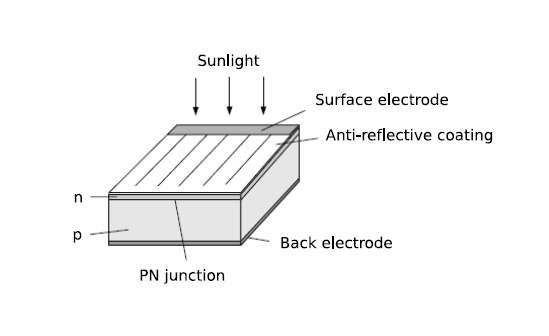
\includegraphics[scale = 0.6]{fig1.png}
	\caption{Structure of crystalline solar cell}
\end{figure}

The figure above shows the structure of a crystalline silicon solar cell.It has 
$n/p$ homo-junctions, a $10 cm \times 10 cm$ p–type silicon plate of thickness $500 \mu m$,
covered with a heavily doped n-type layer with thickness $0.3 \mu m$. The metallic bars on
the n-type layer is one electrode, and a metallic film at the bottom is another. An anti-reflective
film is often applied to reduce the loss of energy reflection.

Photovoltaic Effect describes a process, when the energy of incident photons are absorbed and 
excite electron-hole pairs. Some charges can diffuse to the region of the p-n junction of a 
built-in electric field. Then these charges are drawn to either p-type or n-type area, and thus 
create a photoelectric potential difference.

Solar cells can generate an electric current $I_{ph}$ from the n–type area to the 
p-area based on this effect:

$$
I = I_{ph} - I_{D} = I_{ph} - I_0\left[ exp\left( \frac{qV_D}{nk_BT} \right) -1 \right]
$$

where $V_D$ is the junction voltage, $I_0$ is the diode inverse saturation current, $I_ph$ is the
photocurrent determined by the structure and material characteristics of the solar cell, $I_D$ is 
a forward diode current current from the p-type to the n-type area, $q$ denotes the electron’s charge, $k_B$ is the
Boltzmann’s constant, and $T$ is the temperature in the absolute (Kelvin) scale.

Now we define the fill factor of solar cells $FF$. If $FF$ is bigger, it shows that the output power 
of the solar cell is bigger. This fill factor can be determined by the incident light intensity, the 
forbidden bandwidth, the value of the theoretical coefficient $n$, and the series/parallel resistance.

The fill factor $FF$ can be calculated as:
$$
FF = \frac{P_m}{V_{oc}I_{sc}} = \frac{V_m I_m}{V_{oc}I_{sc}}
$$

We can also define the solar cell energy conversion efficiency $\eta$ as
$$
\eta = \frac{P_m}{P_in} \times 100\%
$$

where $P_{in}$ denotes the total radiant power incident on the solar cell. Now we can plot the 
current-voltage characteristics of a solar cell:

\begin{figure}[H]
	\centering
	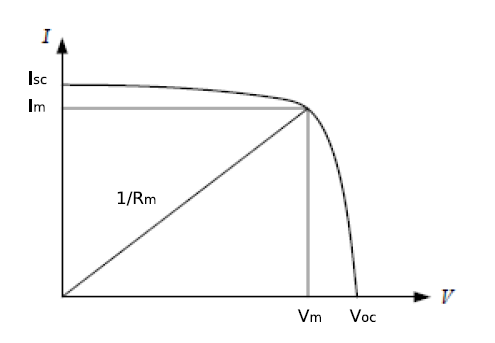
\includegraphics[scale = 0.6]{fig2.png}
	\caption{The current-voltage characteristics of a solar cell.}
\end{figure}

\section{Experimental setup and Measurement procedure}
\subsection{Apparatus}
The setup consists of a photovoltaic device (5 W), a 300 W tungsten–halogen lamp
serving as a radiation source, two digital multimeters, two adjustable resistors, a solar
power meter, a wiring board and a measuring tape.

The multimeter precisions are recorded in "Uncertainty analysis" section.

\subsection{Measurement Procedure}
\subsubsection{I-V characteristics in series/ parallel configuration}
In this part we applied two solar power shells. We first adjust the distance of two 
solar shells to the light source, and make them have almost the same output power. 
Then we connect the two shells in series and in parallel. We also connect some load resistors 
into the circuit. We adjust the resistance of the load resistors and measure the open-circuit 
voltage $V_{oc}$ and short-circuit current $I_{sc}$, and finally plot these data to get a 
I-V characteristics curve.

\subsubsection{I-V characteristics under different solar power input}
In this part, we use only one single solar power shell. We connect a load resistor into the circuit, 
and measure the open-circuit voltage $V_{oc}$ and short-circuit current $I_{sc}$ under different 
resistance values. We also change the distance of the shell to the light source to about $80\%$ of orginal, 
and do exactly the same experiment. Finally we plot two I-V characteristics curves under two different distances.

We also need to measure some other values, such as the size(width and length) of the solar power shell, and 
the power of light measured at different places of the surface of the solar power shell.

\section{Results}
The data sheet is attached to the end of this report.

The uncertainty calculation is included in the next part.

\subsection{I-V characteristics in series/ parallel configuration}
We first measure the solar power input on two solar cells using solar power meter. The 
measured data are listed below:

\begin{table}[H]
	\begin{center}
		\begin{tabular}{|c|c|c|c|c|c|c|}
			\hline
							   & 1   & 2   & 3   & 4   & 5   & 6   \\ \hline
			$P_{84cm} [W/m^2]$ & 366 & 324 & 250 & 246 & 336 & 377 \\ \hline
			$P_{80cm} [W/m^2]$ & 775 & 786 & 669 & 258 & 241 & 218 \\ \hline
			\end{tabular}
			\caption{Measurement data for solar power}
	\end{center}
\end{table}

The measured data taken from my neighbor group might have huge errors. The \\ 
\noindent possible reasons will be discussed in the "Conclusion and discussion" section.\\

We also measure the $I_{sc}$ and $V_{oc}$ of a single solar power shell, and two power shells in 
series and in parallel, without adding any extra resistor. The measured raw data is shown below:
\begin{table}[H]
	\begin{center}
		\begin{tabular}{|l|c|c|c|c|}
		\hline
					  & \multicolumn{1}{l|}{single device at 84 cm} & \multicolumn{1}{l|}{single device at 80 cm} & \multicolumn{1}{l|}{series} & \multicolumn{1}{l|}{parallel} \\ \hline
		$U_{oc} [V]$  & 9.89                                        & 9.82                                        & 19.65                       & 9.83                          \\ \hline
		$I_{sc} [mA]$ & 76.4                                        & 76.5                                        & 77.0                        & 150.5                         \\ \hline
		\end{tabular}
		\caption{Measurement data for $U_{oc}$ and $I_{sc}$}
	\end{center}
\end{table}

So that we can determine the relevant values. For two solar power shells 
connected in series:
\begin{align*}
	U_{oc} &= 19.65\pm 0.11 V \\
	I_{sc} &= 77.0\pm 1.3 mA \\
	U_m &= 16.15\pm 0.09 V \\
	I_m &= 53.7\pm 0.9 mA \\
	P_m &= 867.3 \pm 15.3 mW \\
	R_m &= 301 \pm 5 \Omega \\
	P_{in} &= 22.71 \pm 0.02 W \\
	FF &= 0.573 \pm  0.014 \\
	\eta &= 3.82\% \pm 0.07 \% 
\end{align*}

And for two solar powers connected in parallel:

\begin{align*}
	U_{oc} &= 9.83\pm 0.06 V \\
	I_{sc} &= 150.5\pm 2.4 mA \\
	U_m &= 7.82\pm 0.05 V \\
	I_m &= 116.9\pm 1.9 mA \\
	P_m &= 914.2 \pm 16.0 mW \\
	R_m &= 67 \pm 1 \Omega \\
	P_{in} &= 22.71 \pm 0.02 W \\
	FF &= 0.618 \pm  0.015 \\
	\eta &= 4.02\% \pm 0.07 \% 
\end{align*}

Then we can plot the scatter relations of $I$ vs. $U$ and $P$ vs. $U$:
\begin{figure}[H]
	\centering
	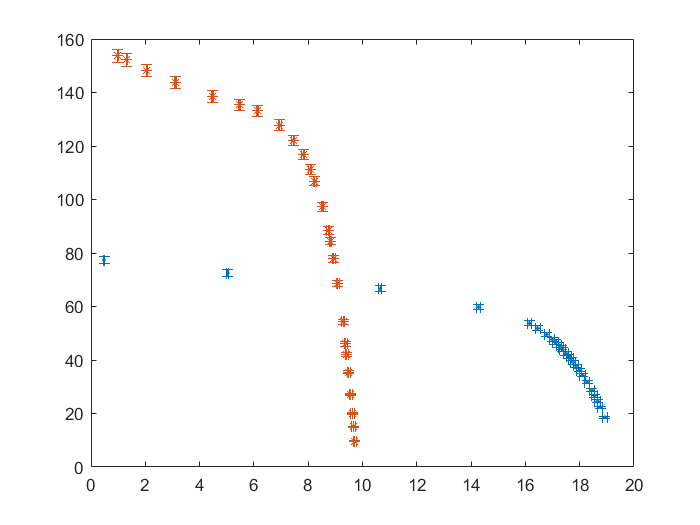
\includegraphics[scale = 0.4]{plot1.png}
	\caption{$I$ vs. $U$ (series/parallel)}
\end{figure}

\begin{figure}[H]
	\centering
	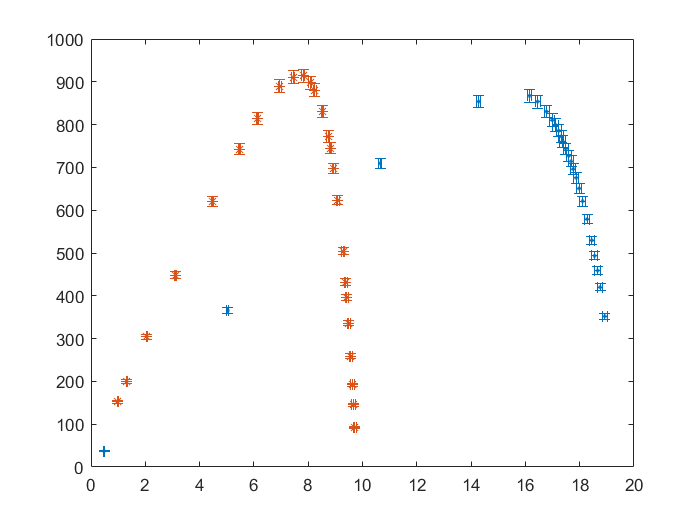
\includegraphics[scale = 0.4]{plot2.png}
	\caption{$P$ vs. $U$ (series/parallel)}
\end{figure}
Note that the red scatters represent for parallel data and blue scatters represent for series data.

The measured and calculated data are listed below:
\begin{table}[H]
	\begin{center}
	\begin{tabular}{|l|llll|llll|}
	\hline
	   & \multicolumn{4}{c|}{series}                                                                           & \multicolumn{4}{c|}{parallel}                                                                           \\ \hline
	   & \multicolumn{1}{l|}{$U[V]$} & \multicolumn{1}{l|}{$I[mA]$} & \multicolumn{1}{l|}{$P[mW]$} & $u_P[mW]$ & \multicolumn{1}{l|}{$U[V]$} & \multicolumn{1}{l|}{$I[mA]$} & \multicolumn{1}{l|}{P{[}mW{]}} & $u_P[mW]$ \\ \hline
	1  & \multicolumn{1}{l|}{0.48}   & \multicolumn{1}{l|}{77.3}    & \multicolumn{1}{l|}{37.1}    & 1.1       & \multicolumn{1}{l|}{9.72}   & \multicolumn{1}{l|}{9.6}     & \multicolumn{1}{l|}{93.3}      & 2.4       \\ \hline
	2  & \multicolumn{1}{l|}{5.04}   & \multicolumn{1}{l|}{72.5}    & \multicolumn{1}{l|}{365.4}   & 6.5       & \multicolumn{1}{l|}{9.67}   & \multicolumn{1}{l|}{15.0}    & \multicolumn{1}{l|}{145.1}     & 3.3       \\ \hline
	3  & \multicolumn{1}{l|}{10.65}  & \multicolumn{1}{l|}{66.6}    & \multicolumn{1}{l|}{709.3}   & 12.4      & \multicolumn{1}{l|}{9.63}   & \multicolumn{1}{l|}{19.9}    & \multicolumn{1}{l|}{191.6}     & 4.0       \\ \hline
	4  & \multicolumn{1}{l|}{14.28}  & \multicolumn{1}{l|}{59.8}    & \multicolumn{1}{l|}{853.9}   & 15.0      & \multicolumn{1}{l|}{9.57}   & \multicolumn{1}{l|}{27.1}    & \multicolumn{1}{l|}{259.3}     & 5.1       \\ \hline
	5  & \multicolumn{1}{l|}{16.15}  & \multicolumn{1}{l|}{53.7}    & \multicolumn{1}{l|}{867.3}   & 15.4      & \multicolumn{1}{l|}{9.50}   & \multicolumn{1}{l|}{35.4}    & \multicolumn{1}{l|}{336.3}     & 6.3       \\ \hline
	6  & \multicolumn{1}{l|}{16.45}  & \multicolumn{1}{l|}{51.9}    & \multicolumn{1}{l|}{853.8}   & 15.2      & \multicolumn{1}{l|}{9.42}   & \multicolumn{1}{l|}{42.1}    & \multicolumn{1}{l|}{396.6}     & 7.3       \\ \hline
	7  & \multicolumn{1}{l|}{16.78}  & \multicolumn{1}{l|}{49.5}    & \multicolumn{1}{l|}{830.6}   & 14.9      & \multicolumn{1}{l|}{9.38}   & \multicolumn{1}{l|}{46.0}    & \multicolumn{1}{l|}{431.5}     & 7.9       \\ \hline
	8  & \multicolumn{1}{l|}{16.99}  & \multicolumn{1}{l|}{47.7}    & \multicolumn{1}{l|}{810.4}   & 14.6      & \multicolumn{1}{l|}{9.29}   & \multicolumn{1}{l|}{54.3}    & \multicolumn{1}{l|}{504.4}     & 9.0       \\ \hline
	9  & \multicolumn{1}{l|}{17.11}  & \multicolumn{1}{l|}{46.7}    & \multicolumn{1}{l|}{799.0}   & 14.4      & \multicolumn{1}{l|}{9.09}   & \multicolumn{1}{l|}{68.6}    & \multicolumn{1}{l|}{623.6}     & 10.9      \\ \hline
	10 & \multicolumn{1}{l|}{17.23}  & \multicolumn{1}{l|}{45.6}    & \multicolumn{1}{l|}{785.7}   & 14.2      & \multicolumn{1}{l|}{8.95}   & \multicolumn{1}{l|}{77.9}    & \multicolumn{1}{l|}{697.2}     & 12.1      \\ \hline
	11 & \multicolumn{1}{l|}{17.32}  & \multicolumn{1}{l|}{44.6}    & \multicolumn{1}{l|}{772.5}   & 14.0      & \multicolumn{1}{l|}{8.82}   & \multicolumn{1}{l|}{84.4}    & \multicolumn{1}{l|}{744.4}     & 12.9      \\ \hline
	12 & \multicolumn{1}{l|}{17.37}  & \multicolumn{1}{l|}{43.8}    & \multicolumn{1}{l|}{760.8}   & 13.8      & \multicolumn{1}{l|}{8.74}   & \multicolumn{1}{l|}{88.4}    & \multicolumn{1}{l|}{772.6}     & 13.3      \\ \hline
	13 & \multicolumn{1}{l|}{17.49}  & \multicolumn{1}{l|}{42.5}    & \multicolumn{1}{l|}{743.3}   & 13.5      & \multicolumn{1}{l|}{8.53}   & \multicolumn{1}{l|}{97.3}    & \multicolumn{1}{l|}{830.0}     & 14.3      \\ \hline
	14 & \multicolumn{1}{l|}{17.60}  & \multicolumn{1}{l|}{41.3}    & \multicolumn{1}{l|}{726.9}   & 13.3      & \multicolumn{1}{l|}{8.24}   & \multicolumn{1}{l|}{106.8}   & \multicolumn{1}{l|}{880.0}     & 15.1      \\ \hline
	15 & \multicolumn{1}{l|}{17.68}  & \multicolumn{1}{l|}{40.4}    & \multicolumn{1}{l|}{714.3}   & 13.1      & \multicolumn{1}{l|}{8.07}   & \multicolumn{1}{l|}{111.2}   & \multicolumn{1}{l|}{897.4}     & 15.3      \\ \hline
	16 & \multicolumn{1}{l|}{17.76}  & \multicolumn{1}{l|}{39.2}    & \multicolumn{1}{l|}{696.2}   & 12.8      & \multicolumn{1}{l|}{7.82}   & \multicolumn{1}{l|}{116.9}   & \multicolumn{1}{l|}{914.2}     & 15.6      \\ \hline
	17 & \multicolumn{1}{l|}{17.87}  & \multicolumn{1}{l|}{37.8}    & \multicolumn{1}{l|}{675.5}   & 12.5      & \multicolumn{1}{l|}{7.45}   & \multicolumn{1}{l|}{122.2}   & \multicolumn{1}{l|}{910.4}     & 15.5      \\ \hline
	18 & \multicolumn{1}{l|}{17.98}  & \multicolumn{1}{l|}{36.2}    & \multicolumn{1}{l|}{650.9}   & 12.1      & \multicolumn{1}{l|}{6.96}   & \multicolumn{1}{l|}{127.8}   & \multicolumn{1}{l|}{889.5}     & 15.2      \\ \hline
	19 & \multicolumn{1}{l|}{18.11}  & \multicolumn{1}{l|}{34.3}    & \multicolumn{1}{l|}{621.2}   & 11.7      & \multicolumn{1}{l|}{6.12}   & \multicolumn{1}{l|}{133.1}   & \multicolumn{1}{l|}{814.6}     & 13.9      \\ \hline
	20 & \multicolumn{1}{l|}{18.27}  & \multicolumn{1}{l|}{31.7}    & \multicolumn{1}{l|}{579.2}   & 11.0      & \multicolumn{1}{l|}{5.48}   & \multicolumn{1}{l|}{135.4}   & \multicolumn{1}{l|}{742.0}     & 12.7      \\ \hline
	21 & \multicolumn{1}{l|}{18.45}  & \multicolumn{1}{l|}{28.7}    & \multicolumn{1}{l|}{529.5}   & 10.2      & \multicolumn{1}{l|}{4.48}   & \multicolumn{1}{l|}{138.5}   & \multicolumn{1}{l|}{620.5}     & 10.7      \\ \hline
	22 & \multicolumn{1}{l|}{18.55}  & \multicolumn{1}{l|}{26.6}    & \multicolumn{1}{l|}{493.4}   & 9.7       & \multicolumn{1}{l|}{3.12}   & \multicolumn{1}{l|}{143.7}   & \multicolumn{1}{l|}{448.3}     & 7.9       \\ \hline
	23 & \multicolumn{1}{l|}{18.66}  & \multicolumn{1}{l|}{24.6}    & \multicolumn{1}{l|}{459.0}   & 9.1       & \multicolumn{1}{l|}{2.05}   & \multicolumn{1}{l|}{148.3}   & \multicolumn{1}{l|}{304.0}     & 5.6       \\ \hline
	24 & \multicolumn{1}{l|}{18.75}  & \multicolumn{1}{l|}{22.4}    & \multicolumn{1}{l|}{420.0}   & 8.5       & \multicolumn{1}{l|}{1.31}   & \multicolumn{1}{l|}{152.2}   & \multicolumn{1}{l|}{199.4}     & 4.0       \\ \hline
	25 & \multicolumn{1}{l|}{18.93}  & \multicolumn{1}{l|}{18.6}    & \multicolumn{1}{l|}{352.1}   & 7.4       & \multicolumn{1}{l|}{0.99}   & \multicolumn{1}{l|}{153.8}   & \multicolumn{1}{l|}{152.3}     & 3.3       \\ \hline
	\end{tabular}
	\caption{Measurement and calculated data for $U$, $I$ and $P$ (series/parallel)}
	\end{center}
\end{table}

\subsection{ I-V characteristics under different solar power input}

We first measure the solar power input on one single solar cell of different distance to light source, using solar power meter.
The measured data are listed below:
\begin{table}[H]
	\begin{center}
	\begin{tabular}{|l|l|l|l|l|l|l|}
	\hline
					   & 1   & 2   & 3   & 4   & 5   & 6   \\ \hline
	$P_{84cm} [W/m^2]$ & 366 & 324 & 250 & 246 & 336 & 377 \\ \hline
	$P_{66cm} [W/m^2]$ & 494 & 231 & 607 & 430 & 196 & 216 \\ \hline
	\end{tabular}
	\caption{Measurement data for solar power}
	\end{center}
\end{table}

So that we can determine the relevant values. For the distance of 84 cm:
\begin{align*}
	U_{oc} &= 9.89 \pm 0.06 V\\
	I_{sc} &= 76.4 \pm 1.2 mA\\
	U_m &= 7.73 \pm 0.05 V\\
	I_m &= 63.4 \pm 1.1 mA\\
	P_m &= 490.1 \pm 9.1 mW\\
	R_m &= 122 \pm 2 \Omega \\
	P_in &= 17.80 \pm 0.02W \\
	FF &= 0.648 \pm 0.016 \\
	\eta &= 2.75 \% \pm 0.05\%
\end{align*}

And for the distance of 66 cm:
\begin{align*}
	U_{oc} &= 9.82 \pm 0.06 V\\
	I_{sc} &= 76.5 \pm 1.2 mA \\
	U_m &= 8.45 \pm 0.05 V \\
	I_m &= 84.5 \pm 1.4 mA\\
	P_m &= 714.0 \pm 12.6 mW\\
	R_m &= 100 \pm 2 \Omega \\
	P_in &= 20.38 \pm 0.02W\\ 
	FF &= 0.950 \pm 0.023\\
	\eta &= 3.50\% \pm 0.06\%
\end{align*}

Then we can plot the scatter relations of $I$ vs. $U$ and $P$ vs. $U$:
\begin{figure}[H]
	\centering
	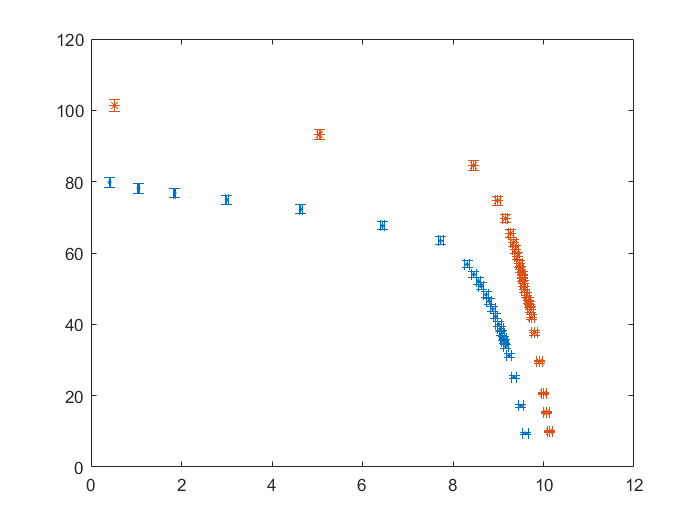
\includegraphics[scale = 0.6]{plot3.png}
	\caption{$I$ vs. $U$ (88cm/66cm)}
\end{figure}

\begin{figure}[H]
	\centering
	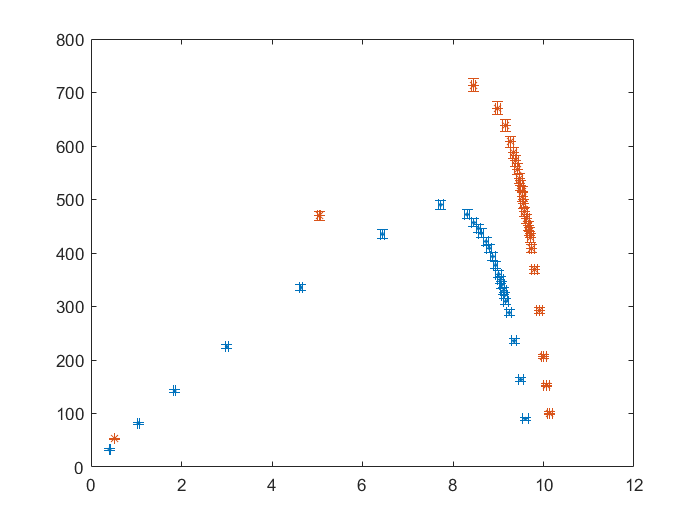
\includegraphics[scale = 0.6]{plot4.png}
	\caption{$P$ vs. $U$ (88cm/66cm)}	
\end{figure}

Note that the red scatters represent for 66 cm data and blue scatters represent for 88 cm data.

The measured and calculated data are listed below:
\begin{table}[H]
	\begin{center}
	\begin{tabular}{|l|llll|llll|}
	\hline
	   & \multicolumn{4}{c|}{66cm}                                                                               & \multicolumn{4}{c|}{84cm}                                                                               \\ \hline
	   & \multicolumn{1}{l|}{$U[V]$} & \multicolumn{1}{l|}{$I[mA]$} & \multicolumn{1}{l|}{P{[}mW{]}} & $u_P[mW]$ & \multicolumn{1}{l|}{$U[V]$} & \multicolumn{1}{l|}{$I[mA]$} & \multicolumn{1}{l|}{P{[}mW{]}} & $u_P[mW]$ \\ \hline
	1  & \multicolumn{1}{l|}{10.14}  & \multicolumn{1}{l|}{9.9}     & \multicolumn{1}{l|}{100.4}     & 2.6       & \multicolumn{1}{l|}{9.60}   & \multicolumn{1}{l|}{9.4}     & \multicolumn{1}{l|}{90.2}      & 2.4       \\ \hline
	2  & \multicolumn{1}{l|}{10.07}  & \multicolumn{1}{l|}{15.2}    & \multicolumn{1}{l|}{153.1}     & 3.4       & \multicolumn{1}{l|}{9.50}   & \multicolumn{1}{l|}{17.2}    & \multicolumn{1}{l|}{163.4}     & 3.5       \\ \hline
	3  & \multicolumn{1}{l|}{10.01}  & \multicolumn{1}{l|}{20.6}    & \multicolumn{1}{l|}{206.2}     & 4.3       & \multicolumn{1}{l|}{9.35}   & \multicolumn{1}{l|}{25.2}    & \multicolumn{1}{l|}{235.6}     & 4.7       \\ \hline
	4  & \multicolumn{1}{l|}{9.91}   & \multicolumn{1}{l|}{29.5}    & \multicolumn{1}{l|}{292.3}     & 5.7       & \multicolumn{1}{l|}{9.24}   & \multicolumn{1}{l|}{31.2}    & \multicolumn{1}{l|}{288.3}     & 5.5       \\ \hline
	5  & \multicolumn{1}{l|}{9.80}   & \multicolumn{1}{l|}{37.6}    & \multicolumn{1}{l|}{368.5}     & 6.9       & \multicolumn{1}{l|}{9.17}   & \multicolumn{1}{l|}{33.8}    & \multicolumn{1}{l|}{309.9}     & 5.9       \\ \hline
	6  & \multicolumn{1}{l|}{9.74}   & \multicolumn{1}{l|}{42.0}    & \multicolumn{1}{l|}{409.1}     & 7.5       & \multicolumn{1}{l|}{9.14}   & \multicolumn{1}{l|}{35.1}    & \multicolumn{1}{l|}{320.8}     & 6.1       \\ \hline
	7  & \multicolumn{1}{l|}{9.71}   & \multicolumn{1}{l|}{44.1}    & \multicolumn{1}{l|}{428.2}     & 7.8       & \multicolumn{1}{l|}{9.12}   & \multicolumn{1}{l|}{36.1}    & \multicolumn{1}{l|}{329.2}     & 6.2       \\ \hline
	8  & \multicolumn{1}{l|}{9.68}   & \multicolumn{1}{l|}{45.5}    & \multicolumn{1}{l|}{440.4}     & 8.0       & \multicolumn{1}{l|}{9.08}   & \multicolumn{1}{l|}{37.5}    & \multicolumn{1}{l|}{340.5}     & 6.4       \\ \hline
	9  & \multicolumn{1}{l|}{9.66}   & \multicolumn{1}{l|}{46.7}    & \multicolumn{1}{l|}{451.1}     & 8.2       & \multicolumn{1}{l|}{9.05}   & \multicolumn{1}{l|}{38.7}    & \multicolumn{1}{l|}{350.2}     & 6.5       \\ \hline
	10 & \multicolumn{1}{l|}{9.63}   & \multicolumn{1}{l|}{48.2}    & \multicolumn{1}{l|}{464.2}     & 8.4       & \multicolumn{1}{l|}{9.01}   & \multicolumn{1}{l|}{40.0}    & \multicolumn{1}{l|}{360.4}     & 6.7       \\ \hline
	11 & \multicolumn{1}{l|}{9.58}   & \multicolumn{1}{l|}{49.8}    & \multicolumn{1}{l|}{477.1}     & 8.6       & \multicolumn{1}{l|}{8.94}   & \multicolumn{1}{l|}{42.2}    & \multicolumn{1}{l|}{377.3}     & 6.9       \\ \hline
	12 & \multicolumn{1}{l|}{9.55}   & \multicolumn{1}{l|}{51.5}    & \multicolumn{1}{l|}{491.8}     & 8.8       & \multicolumn{1}{l|}{8.88}   & \multicolumn{1}{l|}{44.3}    & \multicolumn{1}{l|}{393.4}     & 7.2       \\ \hline
	13 & \multicolumn{1}{l|}{9.54}   & \multicolumn{1}{l|}{52.9}    & \multicolumn{1}{l|}{504.7}     & 9.1       & \multicolumn{1}{l|}{8.80}   & \multicolumn{1}{l|}{46.5}    & \multicolumn{1}{l|}{409.2}     & 7.5       \\ \hline
	14 & \multicolumn{1}{l|}{9.53}   & \multicolumn{1}{l|}{54.0}    & \multicolumn{1}{l|}{514.6}     & 9.2       & \multicolumn{1}{l|}{8.73}   & \multicolumn{1}{l|}{48.3}    & \multicolumn{1}{l|}{421.7}     & 7.7       \\ \hline
	15 & \multicolumn{1}{l|}{9.50}   & \multicolumn{1}{l|}{55.3}    & \multicolumn{1}{l|}{525.4}     & 9.4       & \multicolumn{1}{l|}{8.62}   & \multicolumn{1}{l|}{50.7}    & \multicolumn{1}{l|}{437.0}     & 7.9       \\ \hline
	16 & \multicolumn{1}{l|}{9.47}   & \multicolumn{1}{l|}{57.0}    & \multicolumn{1}{l|}{539.8}     & 9.6       & \multicolumn{1}{l|}{8.56}   & \multicolumn{1}{l|}{52.1}    & \multicolumn{1}{l|}{446.0}     & 8.0       \\ \hline
	17 & \multicolumn{1}{l|}{9.42}   & \multicolumn{1}{l|}{59.1}    & \multicolumn{1}{l|}{556.7}     & 9.9       & \multicolumn{1}{l|}{8.46}   & \multicolumn{1}{l|}{54.0}    & \multicolumn{1}{l|}{456.8}     & 8.2       \\ \hline
	18 & \multicolumn{1}{l|}{9.38}   & \multicolumn{1}{l|}{61.0}    & \multicolumn{1}{l|}{572.2}     & 10.1      & \multicolumn{1}{l|}{8.31}   & \multicolumn{1}{l|}{56.8}    & \multicolumn{1}{l|}{472.0}     & 8.4       \\ \hline
	19 & \multicolumn{1}{l|}{9.34}   & \multicolumn{1}{l|}{62.9}    & \multicolumn{1}{l|}{587.5}     & 10.4      & \multicolumn{1}{l|}{7.73}   & \multicolumn{1}{l|}{63.4}    & \multicolumn{1}{l|}{490.1}     & 8.7       \\ \hline
	20 & \multicolumn{1}{l|}{9.28}   & \multicolumn{1}{l|}{65.5}    & \multicolumn{1}{l|}{607.8}     & 10.7      & \multicolumn{1}{l|}{6.44}   & \multicolumn{1}{l|}{67.6}    & \multicolumn{1}{l|}{435.3}     & 7.7       \\ \hline
	21 & \multicolumn{1}{l|}{9.15}   & \multicolumn{1}{l|}{69.7}    & \multicolumn{1}{l|}{637.8}     & 11.2      & \multicolumn{1}{l|}{4.64}   & \multicolumn{1}{l|}{72.3}    & \multicolumn{1}{l|}{335.5}     & 6.0       \\ \hline
	22 & \multicolumn{1}{l|}{8.99}   & \multicolumn{1}{l|}{74.6}    & \multicolumn{1}{l|}{670.7}     & 11.7      & \multicolumn{1}{l|}{3.00}   & \multicolumn{1}{l|}{74.9}    & \multicolumn{1}{l|}{224.7}     & 4.1       \\ \hline
	23 & \multicolumn{1}{l|}{8.45}   & \multicolumn{1}{l|}{84.5}    & \multicolumn{1}{l|}{714.0}     & 12.4      & \multicolumn{1}{l|}{1.85}   & \multicolumn{1}{l|}{76.8}    & \multicolumn{1}{l|}{142.1}     & 2.7       \\ \hline
	24 & \multicolumn{1}{l|}{5.04}   & \multicolumn{1}{l|}{93.2}    & \multicolumn{1}{l|}{469.7}     & 8.2       & \multicolumn{1}{l|}{1.05}   & \multicolumn{1}{l|}{78.1}    & \multicolumn{1}{l|}{82.0}      & 1.8       \\ \hline
	25 & \multicolumn{1}{l|}{0.52}   & \multicolumn{1}{l|}{101.4}   & \multicolumn{1}{l|}{52.7}      & 1.5       & \multicolumn{1}{l|}{0.41}   & \multicolumn{1}{l|}{79.8}    & \multicolumn{1}{l|}{32.7}      & 1.1       \\ \hline
	\end{tabular}
	\caption{Measured and calculated data for $U$, $I$ and $P$ (66 cm/84 cm)}
	\end{center}
\end{table}

\section{Uncertainty analysis}
The uncertainty caused by multimeter precision limits are listed below:
\begin{table}[H]
	\begin{center}
		\begin{tabular}{|c|c|}
			\hline
			QUANTITY    & PRECISION              \\ \hline
			DC voltage  & $\pm (0.5\%+0.01) [V]$ \\ \hline
			DC current  & $\pm (1.5\%+0.1) [mA]$ \\ \hline
			distance    & $\pm 0.1 [cm]$         \\ \hline
			solar power & $\pm 10 [w/m^2]$       \\ \hline
			\end{tabular}
			\caption{Multimeter precision}
	\end{center}
\end{table}

So that the uncertainties for raw data can be calculated as:

\begin{table}[H]
	\begin{center}
	\begin{tabular}{|l|llll|llll|}
	\hline
	   & \multicolumn{4}{c|}{series}                                                                            & \multicolumn{4}{c|}{parallel}                                                                          \\ \hline
	   & \multicolumn{1}{l|}{$U[V]$} & \multicolumn{1}{l|}{$u_U[V]$} & \multicolumn{1}{l|}{$I[mA]$} & $u_I[mA]$ & \multicolumn{1}{l|}{$U[V]$} & \multicolumn{1}{l|}{$u_U[V]$} & \multicolumn{1}{l|}{$I[mA]$} & $u_I[mA]$ \\ \hline
	1  & \multicolumn{1}{l|}{0.48}   & \multicolumn{1}{l|}{0.01}     & \multicolumn{1}{l|}{77.3}    & 1.3       & \multicolumn{1}{l|}{9.72}   & \multicolumn{1}{l|}{0.06}     & \multicolumn{1}{l|}{9.6}     & 0.2       \\ \hline
	2  & \multicolumn{1}{l|}{5.04}   & \multicolumn{1}{l|}{0.04}     & \multicolumn{1}{l|}{72.5}    & 1.2       & \multicolumn{1}{l|}{9.67}   & \multicolumn{1}{l|}{0.06}     & \multicolumn{1}{l|}{15.0}    & 0.3       \\ \hline
	3  & \multicolumn{1}{l|}{10.65}  & \multicolumn{1}{l|}{0.06}     & \multicolumn{1}{l|}{66.6}    & 1.1       & \multicolumn{1}{l|}{9.63}   & \multicolumn{1}{l|}{0.06}     & \multicolumn{1}{l|}{19.9}    & 0.4       \\ \hline
	4  & \multicolumn{1}{l|}{14.28}  & \multicolumn{1}{l|}{0.08}     & \multicolumn{1}{l|}{59.8}    & 1.0       & \multicolumn{1}{l|}{9.57}   & \multicolumn{1}{l|}{0.06}     & \multicolumn{1}{l|}{27.1}    & 0.5       \\ \hline
	5  & \multicolumn{1}{l|}{16.15}  & \multicolumn{1}{l|}{0.09}     & \multicolumn{1}{l|}{53.7}    & 0.9       & \multicolumn{1}{l|}{9.50}   & \multicolumn{1}{l|}{0.06}     & \multicolumn{1}{l|}{35.4}    & 0.6       \\ \hline
	6  & \multicolumn{1}{l|}{16.45}  & \multicolumn{1}{l|}{0.09}     & \multicolumn{1}{l|}{51.9}    & 0.9       & \multicolumn{1}{l|}{9.42}   & \multicolumn{1}{l|}{0.06}     & \multicolumn{1}{l|}{42.1}    & 0.7       \\ \hline
	7  & \multicolumn{1}{l|}{16.78}  & \multicolumn{1}{l|}{0.09}     & \multicolumn{1}{l|}{49.5}    & 0.8       & \multicolumn{1}{l|}{9.38}   & \multicolumn{1}{l|}{0.06}     & \multicolumn{1}{l|}{46.0}    & 0.8       \\ \hline
	8  & \multicolumn{1}{l|}{16.99}  & \multicolumn{1}{l|}{0.09}     & \multicolumn{1}{l|}{47.7}    & 0.8       & \multicolumn{1}{l|}{9.29}   & \multicolumn{1}{l|}{0.06}     & \multicolumn{1}{l|}{54.3}    & 0.9       \\ \hline
	9  & \multicolumn{1}{l|}{17.11}  & \multicolumn{1}{l|}{0.10}     & \multicolumn{1}{l|}{46.7}    & 0.8       & \multicolumn{1}{l|}{9.09}   & \multicolumn{1}{l|}{0.06}     & \multicolumn{1}{l|}{68.6}    & 1.1       \\ \hline
	10 & \multicolumn{1}{l|}{17.23}  & \multicolumn{1}{l|}{0.10}     & \multicolumn{1}{l|}{45.6}    & 0.8       & \multicolumn{1}{l|}{8.95}   & \multicolumn{1}{l|}{0.05}     & \multicolumn{1}{l|}{77.9}    & 1.3       \\ \hline
	11 & \multicolumn{1}{l|}{17.32}  & \multicolumn{1}{l|}{0.10}     & \multicolumn{1}{l|}{44.6}    & 0.8       & \multicolumn{1}{l|}{8.82}   & \multicolumn{1}{l|}{0.05}     & \multicolumn{1}{l|}{84.4}    & 1.4       \\ \hline
	12 & \multicolumn{1}{l|}{17.37}  & \multicolumn{1}{l|}{0.10}     & \multicolumn{1}{l|}{43.8}    & 0.8       & \multicolumn{1}{l|}{8.74}   & \multicolumn{1}{l|}{0.05}     & \multicolumn{1}{l|}{88.4}    & 1.4       \\ \hline
	13 & \multicolumn{1}{l|}{17.49}  & \multicolumn{1}{l|}{0.10}     & \multicolumn{1}{l|}{42.5}    & 0.7       & \multicolumn{1}{l|}{8.53}   & \multicolumn{1}{l|}{0.05}     & \multicolumn{1}{l|}{97.3}    & 1.6       \\ \hline
	14 & \multicolumn{1}{l|}{17.60}  & \multicolumn{1}{l|}{0.10}     & \multicolumn{1}{l|}{41.3}    & 0.7       & \multicolumn{1}{l|}{8.24}   & \multicolumn{1}{l|}{0.05}     & \multicolumn{1}{l|}{106.8}   & 1.7       \\ \hline
	15 & \multicolumn{1}{l|}{17.68}  & \multicolumn{1}{l|}{0.10}     & \multicolumn{1}{l|}{40.4}    & 0.7       & \multicolumn{1}{l|}{8.07}   & \multicolumn{1}{l|}{0.05}     & \multicolumn{1}{l|}{111.2}   & 1.8       \\ \hline
	16 & \multicolumn{1}{l|}{17.76}  & \multicolumn{1}{l|}{0.10}     & \multicolumn{1}{l|}{39.2}    & 0.7       & \multicolumn{1}{l|}{7.82}   & \multicolumn{1}{l|}{0.05}     & \multicolumn{1}{l|}{116.9}   & 1.9       \\ \hline
	17 & \multicolumn{1}{l|}{17.87}  & \multicolumn{1}{l|}{0.10}     & \multicolumn{1}{l|}{37.8}    & 0.7       & \multicolumn{1}{l|}{7.45}   & \multicolumn{1}{l|}{0.05}     & \multicolumn{1}{l|}{122.2}   & 1.9       \\ \hline
	18 & \multicolumn{1}{l|}{17.98}  & \multicolumn{1}{l|}{0.10}     & \multicolumn{1}{l|}{36.2}    & 0.6       & \multicolumn{1}{l|}{6.96}   & \multicolumn{1}{l|}{0.04}     & \multicolumn{1}{l|}{127.8}   & 2.0       \\ \hline
	19 & \multicolumn{1}{l|}{18.11}  & \multicolumn{1}{l|}{0.10}     & \multicolumn{1}{l|}{34.3}    & 0.6       & \multicolumn{1}{l|}{6.12}   & \multicolumn{1}{l|}{0.04}     & \multicolumn{1}{l|}{133.1}   & 2.1       \\ \hline
	20 & \multicolumn{1}{l|}{18.27}  & \multicolumn{1}{l|}{0.10}     & \multicolumn{1}{l|}{31.7}    & 0.6       & \multicolumn{1}{l|}{5.48}   & \multicolumn{1}{l|}{0.04}     & \multicolumn{1}{l|}{135.4}   & 2.1       \\ \hline
	21 & \multicolumn{1}{l|}{18.45}  & \multicolumn{1}{l|}{0.10}     & \multicolumn{1}{l|}{28.7}    & 0.5       & \multicolumn{1}{l|}{4.48}   & \multicolumn{1}{l|}{0.03}     & \multicolumn{1}{l|}{138.5}   & 2.2       \\ \hline
	22 & \multicolumn{1}{l|}{18.55}  & \multicolumn{1}{l|}{0.10}     & \multicolumn{1}{l|}{26.6}    & 0.5       & \multicolumn{1}{l|}{3.12}   & \multicolumn{1}{l|}{0.03}     & \multicolumn{1}{l|}{143.7}   & 2.3       \\ \hline
	23 & \multicolumn{1}{l|}{18.66}  & \multicolumn{1}{l|}{0.10}     & \multicolumn{1}{l|}{24.6}    & 0.5       & \multicolumn{1}{l|}{2.05}   & \multicolumn{1}{l|}{0.02}     & \multicolumn{1}{l|}{148.3}   & 2.3       \\ \hline
	24 & \multicolumn{1}{l|}{18.75}  & \multicolumn{1}{l|}{0.10}     & \multicolumn{1}{l|}{22.4}    & 0.4       & \multicolumn{1}{l|}{1.31}   & \multicolumn{1}{l|}{0.02}     & \multicolumn{1}{l|}{152.2}   & 2.4       \\ \hline
	25 & \multicolumn{1}{l|}{18.93}  & \multicolumn{1}{l|}{0.10}     & \multicolumn{1}{l|}{18.6}    & 0.4       & \multicolumn{1}{l|}{0.99}   & \multicolumn{1}{l|}{0.01}     & \multicolumn{1}{l|}{153.8}   & 2.4       \\ \hline
	\end{tabular}
	\caption{Measurement and uncertainties for $U$ vs. $I$ (series/parallel)}		
	\end{center}
\end{table}

\begin{table}[H]
	\begin{center}
	\begin{tabular}{|l|llll|llll|}
	\hline
	   & \multicolumn{4}{c|}{66cm}                                                                              & \multicolumn{4}{c|}{84cm}                                                                              \\ \hline
	   & \multicolumn{1}{l|}{$U[V]$} & \multicolumn{1}{l|}{$u_U[V]$} & \multicolumn{1}{l|}{$I[mA]$} & $u_I[mA]$ & \multicolumn{1}{l|}{$U[V]$} & \multicolumn{1}{l|}{$u_U[V]$} & \multicolumn{1}{l|}{$I[mA]$} & $u_I[mA]$ \\ \hline
	1  & \multicolumn{1}{l|}{10.14}  & \multicolumn{1}{l|}{0.06}     & \multicolumn{1}{l|}{9.9}     & 0.2       & \multicolumn{1}{l|}{9.60}   & \multicolumn{1}{l|}{0.06}     & \multicolumn{1}{l|}{9.4}     & 0.2       \\ \hline
	2  & \multicolumn{1}{l|}{10.07}  & \multicolumn{1}{l|}{0.06}     & \multicolumn{1}{l|}{15.2}    & 0.3       & \multicolumn{1}{l|}{9.50}   & \multicolumn{1}{l|}{0.06}     & \multicolumn{1}{l|}{17.2}    & 0.4       \\ \hline
	3  & \multicolumn{1}{l|}{10.01}  & \multicolumn{1}{l|}{0.06}     & \multicolumn{1}{l|}{20.6}    & 0.4       & \multicolumn{1}{l|}{9.35}   & \multicolumn{1}{l|}{0.06}     & \multicolumn{1}{l|}{25.2}    & 0.5       \\ \hline
	4  & \multicolumn{1}{l|}{9.91}   & \multicolumn{1}{l|}{0.06}     & \multicolumn{1}{l|}{29.5}    & 0.5       & \multicolumn{1}{l|}{9.24}   & \multicolumn{1}{l|}{0.06}     & \multicolumn{1}{l|}{31.2}    & 0.6       \\ \hline
	5  & \multicolumn{1}{l|}{9.80}   & \multicolumn{1}{l|}{0.06}     & \multicolumn{1}{l|}{37.6}    & 0.7       & \multicolumn{1}{l|}{9.17}   & \multicolumn{1}{l|}{0.06}     & \multicolumn{1}{l|}{33.8}    & 0.6       \\ \hline
	6  & \multicolumn{1}{l|}{9.74}   & \multicolumn{1}{l|}{0.06}     & \multicolumn{1}{l|}{42.0}    & 0.7       & \multicolumn{1}{l|}{9.14}   & \multicolumn{1}{l|}{0.06}     & \multicolumn{1}{l|}{35.1}    & 0.6       \\ \hline
	7  & \multicolumn{1}{l|}{9.71}   & \multicolumn{1}{l|}{0.06}     & \multicolumn{1}{l|}{44.1}    & 0.8       & \multicolumn{1}{l|}{9.12}   & \multicolumn{1}{l|}{0.06}     & \multicolumn{1}{l|}{36.1}    & 0.6       \\ \hline
	8  & \multicolumn{1}{l|}{9.68}   & \multicolumn{1}{l|}{0.06}     & \multicolumn{1}{l|}{45.5}    & 0.8       & \multicolumn{1}{l|}{9.08}   & \multicolumn{1}{l|}{0.06}     & \multicolumn{1}{l|}{37.5}    & 0.7       \\ \hline
	9  & \multicolumn{1}{l|}{9.66}   & \multicolumn{1}{l|}{0.06}     & \multicolumn{1}{l|}{46.7}    & 0.8       & \multicolumn{1}{l|}{9.05}   & \multicolumn{1}{l|}{0.06}     & \multicolumn{1}{l|}{38.7}    & 0.7       \\ \hline
	10 & \multicolumn{1}{l|}{9.63}   & \multicolumn{1}{l|}{0.06}     & \multicolumn{1}{l|}{48.2}    & 0.8       & \multicolumn{1}{l|}{9.01}   & \multicolumn{1}{l|}{0.06}     & \multicolumn{1}{l|}{40.0}    & 0.7       \\ \hline
	11 & \multicolumn{1}{l|}{9.58}   & \multicolumn{1}{l|}{0.06}     & \multicolumn{1}{l|}{49.8}    & 0.8       & \multicolumn{1}{l|}{8.94}   & \multicolumn{1}{l|}{0.05}     & \multicolumn{1}{l|}{42.2}    & 0.7       \\ \hline
	12 & \multicolumn{1}{l|}{9.55}   & \multicolumn{1}{l|}{0.06}     & \multicolumn{1}{l|}{51.5}    & 0.9       & \multicolumn{1}{l|}{8.88}   & \multicolumn{1}{l|}{0.05}     & \multicolumn{1}{l|}{44.3}    & 0.8       \\ \hline
	13 & \multicolumn{1}{l|}{9.54}   & \multicolumn{1}{l|}{0.06}     & \multicolumn{1}{l|}{52.9}    & 0.9       & \multicolumn{1}{l|}{8.80}   & \multicolumn{1}{l|}{0.05}     & \multicolumn{1}{l|}{46.5}    & 0.8       \\ \hline
	14 & \multicolumn{1}{l|}{9.53}   & \multicolumn{1}{l|}{0.06}     & \multicolumn{1}{l|}{54.0}    & 0.9       & \multicolumn{1}{l|}{8.73}   & \multicolumn{1}{l|}{0.05}     & \multicolumn{1}{l|}{48.3}    & 0.8       \\ \hline
	15 & \multicolumn{1}{l|}{9.50}   & \multicolumn{1}{l|}{0.06}     & \multicolumn{1}{l|}{55.3}    & 0.9       & \multicolumn{1}{l|}{8.62}   & \multicolumn{1}{l|}{0.05}     & \multicolumn{1}{l|}{50.7}    & 0.9       \\ \hline
	16 & \multicolumn{1}{l|}{9.47}   & \multicolumn{1}{l|}{0.06}     & \multicolumn{1}{l|}{57.0}    & 1.0       & \multicolumn{1}{l|}{8.56}   & \multicolumn{1}{l|}{0.05}     & \multicolumn{1}{l|}{52.1}    & 0.9       \\ \hline
	17 & \multicolumn{1}{l|}{9.42}   & \multicolumn{1}{l|}{0.06}     & \multicolumn{1}{l|}{59.1}    & 1.0       & \multicolumn{1}{l|}{8.46}   & \multicolumn{1}{l|}{0.05}     & \multicolumn{1}{l|}{54.0}    & 0.9       \\ \hline
	18 & \multicolumn{1}{l|}{9.38}   & \multicolumn{1}{l|}{0.06}     & \multicolumn{1}{l|}{61.0}    & 1.0       & \multicolumn{1}{l|}{8.31}   & \multicolumn{1}{l|}{0.05}     & \multicolumn{1}{l|}{56.8}    & 1.0       \\ \hline
	19 & \multicolumn{1}{l|}{9.34}   & \multicolumn{1}{l|}{0.06}     & \multicolumn{1}{l|}{62.9}    & 1.0       & \multicolumn{1}{l|}{7.73}   & \multicolumn{1}{l|}{0.05}     & \multicolumn{1}{l|}{63.4}    & 1.1       \\ \hline
	20 & \multicolumn{1}{l|}{9.28}   & \multicolumn{1}{l|}{0.06}     & \multicolumn{1}{l|}{65.5}    & 1.1       & \multicolumn{1}{l|}{6.44}   & \multicolumn{1}{l|}{0.04}     & \multicolumn{1}{l|}{67.6}    & 1.1       \\ \hline
	21 & \multicolumn{1}{l|}{9.15}   & \multicolumn{1}{l|}{0.06}     & \multicolumn{1}{l|}{69.7}    & 1.1       & \multicolumn{1}{l|}{4.64}   & \multicolumn{1}{l|}{0.03}     & \multicolumn{1}{l|}{72.3}    & 1.2       \\ \hline
	22 & \multicolumn{1}{l|}{8.99}   & \multicolumn{1}{l|}{0.05}     & \multicolumn{1}{l|}{74.6}    & 1.2       & \multicolumn{1}{l|}{3.00}   & \multicolumn{1}{l|}{0.03}     & \multicolumn{1}{l|}{74.9}    & 1.2       \\ \hline
	23 & \multicolumn{1}{l|}{8.45}   & \multicolumn{1}{l|}{0.05}     & \multicolumn{1}{l|}{84.5}    & 1.4       & \multicolumn{1}{l|}{1.85}   & \multicolumn{1}{l|}{0.02}     & \multicolumn{1}{l|}{76.8}    & 1.3       \\ \hline
	24 & \multicolumn{1}{l|}{5.04}   & \multicolumn{1}{l|}{0.04}     & \multicolumn{1}{l|}{93.2}    & 1.5       & \multicolumn{1}{l|}{1.05}   & \multicolumn{1}{l|}{0.02}     & \multicolumn{1}{l|}{78.1}    & 1.3       \\ \hline
	25 & \multicolumn{1}{l|}{0.52}   & \multicolumn{1}{l|}{0.01}     & \multicolumn{1}{l|}{101.4}   & 1.6       & \multicolumn{1}{l|}{0.41}   & \multicolumn{1}{l|}{0.01}     & \multicolumn{1}{l|}{79.8}    & 1.3       \\ \hline
	\end{tabular}
	\caption{Measurement and uncertainties for $U$ vs. $I$ (66cm/84cm)}
	\end{center}
\end{table}

\subsection{Uncertainty of Power $P$}
Since we have $P = U \times I$, we can calculate its uncertainty through:
$$
u_P = \sqrt{(\frac{\partial P}{\partial U}u_U)^2 + (\frac{\partial P}{\partial I}u_I)^2} = \sqrt{(I\cdot u_U)^2 + (U \cdot u_I)^2}
$$

When $I = 53.7 \pm 0.9 mA$ and $U = 16.15 \pm 0.09 V$, the calculation is:
\begin{align*}
	P &= UI = 53.7 \cdot 16.15 = 867.3 mW \\
	u_P &= \sqrt{(53.7 \cdot 0.09)^2 + (16.15 \cdot 0.9)^2} = 15.3 mW
\end{align*}

So that $P = 867.3 \pm 15.3 mW$

\subsection{Uncertainty of Resistance $R$}
Since we have $R = U/I$, we can calculate the uncertainty through:
$$
u_R = \sqrt{(\frac{\partial R}{\partial U} u_U)^2 + (\frac{\partial R}{\partial I} u_I)^2} = R \sqrt{(\frac{u_U}{U})^2 + (\frac{u_I}{I})^2}
$$

When $I = 53.7 \pm 0.9 mA$ and $U = 16.15 \pm 0.09 V$, the calculation is:
\begin{align*}
	R &= U/I = 16.15/(53.7/1000) = 301 \Omega \\
	u_R &= 301 \cdot \sqrt{(0.09/16.15)^2 + (0.9/53.7)^2} = 5 \Omega
\end{align*}

So that $R = 301 \pm 5 \Omega$

\subsection{Uncertainty of Fill Factor $FF$}
Since we have $FF = P_m/(U_{oc}\cdot I_{sc}) = (U_m \cdot I_m)/(U_{oc} \cdot I_{sc})$, we can calculate the uncertainty through:
\begin{align*}
u_{FF} &= \sqrt{(\frac{\partial FF}{\partial P_m} u_{P_m})^2 + (\frac{\partial FF}{\partial U_{oc}}u_{U_{oc}})^2 + (\frac{\partial FF}{\partial I_{sc}}u_{I_{sc}})^2}
	\\ &= FF \sqrt{(\frac{u_{U_m}}{U_m})^2 + (\frac{u_{I_m}}{I_m})^2 + (\frac{u_{U_{oc}}}{U_{oc}})^2 + (\frac{u_{I_{sc}}}{I_{sc}})^2}
\end{align*}

When $U_{oc} = 19.65\pm 0.11 V$, $I_{sc} = 77.0\pm 1.3 mA$, $U_m = 16.15\pm 0.09 V$, $I_m = 53.7\pm 0.9 mA$, the calculation is:

\begin{align*}
	FF &= \frac{16.15 \cdot 53.7}{19.65 \cdot 77.0} = 0.573 \\
	u_{FF} &= 0.573 \cdot \sqrt{(0.09/16.15)^2 + (0.9/53.7)^2 + (0.11/19.65)^2 + (1.3/77.0)^2} \\
	       &= 0.014
\end{align*}

So that $FF = 0.573 \pm 0.014$

\subsection{Uncertainty of Energy Conversion Efficiency $\eta$}
Since we have $\eta = U_m \cdot I_m /P_{in}$, we can calculate the uncertainty through:
\begin{align*}
	u_{\eta} &= \sqrt{(\frac{\partial \eta}{\partial U_m} u_{U_m})^2 + (\frac{\partial \eta}{\partial I_m}u_{I_m})^2 + (\frac{\partial \eta}{\partial P_{in}} u_{P_{in}})^2} \\
			 &= \eta \sqrt{(\frac{u_{I_m}}{I_m})^2 + (\frac{u_{U_m}}{U_m})^2 + (\frac{u_{P_{in}}}{P_{in}})^2}
\end{align*}

When $U_m = 16.15\pm 0.09 V $, $I_m = 53.7\pm 0.9 mA$, $P_{in} = 22.71 \pm 0.02 W $, the calculation is:
\begin{align*}
	\eta &= 16.15 \cdot 53.7 / 1000 / 22.71 = 3.82 \% \\
	u_{\eta} &= 3.82\% \cdot \sqrt{(0.9/53.7)^2+(0.09/16.15)^2+(0.02/22.71)^2} \\
	         &= 0.07\%
\end{align*}

So that $\eta = 3.82\% \pm 0.07 \%$

\section{Conclusion and discussion}
In this lab we explored the  I-V characteristics of the solar power cell of different configurations. We did the 
experiment by connecting two solar power shells of similar output powers in series and in parallel, and by one single 
solar power shell with two different distance to the light source. We also connect a 
resistor into the circuit and change its resistance widly, and measure the short-circuit current 
$I_{sc}$ and the open-circuit voltage $V_{oc}$. Finally we calculate the maximum output power $P_m$, the power factor 
$FF$, the energy conversion efficiency $\eta$, and we plot the graphs of $I$ vs. $U$ and 
$P$ vs. $U$ to find their relations.

There are a lot of reasons that might cause huge uncertainties. In the first section involving two solar power shells, 
the light source of two neighbor groups are so close to each other, that the light of one group can easily cover the solar 
power shell of the neighbor group, and thus greatly affect the experiment data. I also find that the measurement data 
for solar power recorded from my neighbor group is very weird and varies largely. This is possibly because their light source 
did not face perpendicularly to the solar power shell, so that the middle of the solar power shell actually gets 
less light than one of its corner.

In section two involving one single solar power shell, I recorded the data for $U_{oc}$ and $I_{sc}$ wrongly. I should have 
recorded the data with distance of 66 cm, but I measured them at 80 cm. This made both $U_{oc}$ and $I_{sc}$ smaller than 
theoretical data, and eventually it made the $FF$ very big. So this unreasonable result is actually caused by measurement mistake. 

To inprove the experiment, we can insert a pure black plastic board between groups. This board can not only prevent the light 
from other groups from dusturbing the solar power shell, but also absorbe extra light and prevent light reflection. It is also better 
to pull down the curtain and turn off indoor lights, to prevent all extra light sources from disturbing.

Regardless of these two sets of data mentioned above, all other data are quite reasonable, with relatively small errors. We can see 
than when the light source is closer to the solar power shell, more power are absorbed and thus the power produced is bigger. The four 
plotted graphs are also quite match with that introduced in lab manual, witch indicates that the experiment is quite successful overal, 
and the experiment data indicates the theory is correct.

\section{References}
    \begin{enumerate}
        \item Qin Tian, Cao Jianjun, Yi Hankun, Wu Ziyou, Zhang Yifei, Yao Yuan, Mateusz Krzyzosiak
    \end{enumerate}

\end{document}
